\begin{savequote}[75mm]
Do not lose your faith. A mighty fortress is our mathematics. It shall rise to the occasion. It always has. 
\qauthor{Stanislaw Ulam (1909-1984)}
\end{savequote}

\chapter{Selecting Suitable Sites}
\label{chapter 1}

\newpage

\section{Software Availability}

The software tools developed as part of this research program are freely available as a GitHub repository hosted at the following URL: \url{https://github.com/ericdfournier/WOGRSS}. The repository title acronym WOGRSS stands for: Weighted Overlay Groundwater Recharge Site Suitability model. The software has been developed using MATLAB$^{\circledR}$ a multi-paradigm, imperative, procedural language that is commonly used for numerical scientific computing \cite{MATLAB2013}. The provided tools can be used in one of two ways. The first is as a library of functions which can be selectively integrated into other MATLAB$^{\circledR}$ based modeling workflows. The second is as a packaged executable with a graphical user interface that allow for more facile, independent use. 
 
\section{Multi-Criteria Site Suitability Analyses}

Multi-criteria site suitability (MCSS) analyses involve the combination of two or more input geographic data layers that each correspond to some independent measure of site suitability for a given landuse application \cite{Bolstad2005}. The output of an MCSS computation is a single geographic data layer in which the value at each location represents a composite measure of overall site suitability relative to all of the independent criteria, simultaneously \cite{Hopkins1977, Collins2001}. MCSS are typically conducted using geographic information that has been stored in a raster format. This means that prior to conducting this type of analysis each of the input geographic data layers that are to be used must be preprocessed relative to some reference raster format so as to ensure the feasibility and consistency of the MCSS computation. For example, in order for the computation to be feasible: all of the input data layers must have the same number of cells and occupy that same geographic extent. Similarly, in order for the computation to be consistent: the ordinality and the scaling of the values in each raster must accurately reflect the relative weighting and directionality of each independent suitability criterium.
 
Geographic information system (GIS) software packages are commonly used to conduct both these types of data preprocessing operations as well as the MCSS computation itself \cite{Malczewski2004, Malczewski2006}. This is because they provide pre-built functions which readily facilitate the import of spatial data layers from disparate sources as well as the manipulation of geographic data layers such that they satisfy the previously mentioned feasibility and consistency constraints. It is often the case however, that the MCSS analyses itself is not the endpoint goal of a given research effort. Many times, the output of MCSS analyses are used as inputs to some other, more complex, numerical optimization model \cite{Church2002}. This situation is frequently encountered in the fields of operations research (OR) and location science (LS) where MCSS outputs are used to derive network topologies or linear programming constraints for optimization problems related to vehicle routing, flow maximization, or facility location \cite{Huber1985, Church1992}. 

Unfortunately, legacy software development issues have heretofore prevented the tight integration of GIS based MCSS modeling workflows with these other types of OR \& LS domain specific numerical routines \cite{Church2002}. Recently improvements in both commercial as well as open source software packages however, have begun to transform this situation, enabling a much tighter coupling of spatial data processing operations with spatially explicit numerical models. In light of these recent advances, this paper introduces a set of software tools, written in the MATLAB$^{\circledR}$ programming language, which demonstrates how many of the operations associated with MCSS analyses that would typically be conducted within a GIS software system, can now be readily accomplished within the same computational environment that is popularly used for general purpose numerical computing. The capabilities of this toolset are exposed in this note via a case study implementation involving the preprocessing of multiple geographic data layers for an MCSS problem involving the siting of locations for the artificial recharge of groundwater resources. This particular MCSS problem has been selected to illustrate the toolset's capability to handle diverse input data sources which span an effective geographic domain comprising the entire state of California.

\section{Siting Infrastructure for Artificial Groundwater Recharge}
    
As mentioned previously, the case study MCSS model which shall be referenced pertains tot the location of suitable sites for the artificial recharge of groundwater recharge in the State of California. It is estimated that one third of the potable water delivered by public utilities in the United States (US) is drawn from subsurface aquifers \cite{Hutson2004}. Additionally, recent data collected by the USGS indicate that a full 98\% of self-supplied domestic water withdrawals in the US come from groundwater resources as well \cite{Maupin2014}. Despite this  continued reliance on the availability of high quality groundwater resources, regional trends toward growth in both the volume of freshwater demand as well as uncertainty in the spatio-temporal distribution of supply have caused groundwater resources in many parts of the US, as well as elsewhere around the world, to become critically oversubscribed \cite{Karl2009, Wada2010}. The gravity of this situation has been further compounded in heavily urbanized regions where large areas of impervious surfaces can prevent the natural recharge of subsurface aquifers \cite{Shuster2005, Seiler2007}.

Beyond the loss of water available for various beneficial uses, unsustainable use of groundwater resources can result in a number of debilitating long term consequences including: land subsidence, well depletion, and in coastal areas, seawater intrusion into freshwater aquifers \cite{NRC2008, Gleeson2012}. As a result, water resource managers are increasingly turning to artificial groundwater recharge projects in an effort to augment recharge rates and mitigate these types of harmful long term effects associated with prolonged oversubscription \cite{Dillon2005,  Langridge2012, NRC2012}.

The two most commonly implemented artificial groundwater recharge applications are spreading basins and direct injection wells \cite{Asano1985, Bouwer1999}. Spreading basins operate by passively transporting of water from the surface to the subsurface under the force of gravity through an unsaturated permeable soil layer \cite{Pyne1995, Asano1998}. These types of artificial basins are typically constructed by excavating a region whose existing surface geomorphology provides good hydraulic connectivity to the aquifer that is to be recharged \cite{Marino1975a, Marino1975b}. Alternatively, direct injection wells operate by actively transporting water from the surface to the subsurface under mechanized pump force downwards through the shaft of vertical bore hole \cite{USEPA2001}. In the case of direct injection wells, the bore hole must be drilled to a depth that makes contact with the aquifer that is to be recharged. Furthermore, direct injection wells require the continuous operation of some sort of pump mechanism in order to maintain the pressure head required to force water through the pore spaces within the aquifer and, in some instances, against an existing hydraulic gradient \cite{Bouwer1991}.

These different artificial recharge applications tend to be implemented mutually exclusively due to their contrasting operational characteristics \cite{Asano1998, NRC2008, NRC2012}. For example, spreading basins tend to have relatively high upfront costs, due to the need for land acquisition and excavation; however, they also tend to have low operation and maintenance fees, due to the simplicity of the gravity fed system and the limited need for anti-fowling measures associated caused by the modest rates of infiltration \cite{Bouwer1999, Bouwer2002, Todd2005}. Conversely, direct injection wells tend to have relatively lower upfront costs, due to the minimal land requirements and construction costs associated with individual wells; however, they also tend to have high operation and maintenance fees, due to the need to supply continuous pump energy as well as to apply significant anti-fowling measures because of the relatively high rates of infiltration \cite{Pyne1995, Bouwer1999, Bouwer2002}.

Previous MCSS models which have sought to rank potential sites for both types of artificial groundwater recharge applications have shown that there is a need to take into account a large number of factors ranging from natural physical attributes of the landscape such as: elevation, slope, surface geology, and soil composition to things like administrative boundaries or the location of existing civil infrastructure components like streets, highways, and surface water impoundments \cite{Kallali2007, Ghayoumian2007, Pedrero2011, Sargaonkar2011, Albuquerque2012, Rahman2012}. These previous studies have shown that the data preprocessing workflow which involves aligning and aggregating such a diverse set of input spatial data sources can constitute a substantial fraction of the effort associated with the entire analyses. 

\section{Data Preprocessing}
    
The generic data preprocessing workflow for most any MCSS analysis involves one or more of the three phases illustrated conceptually in ~Figure \ref{fig:Preprocessing}. First, all of the input spatial data layers must be checked to determine whether or not they possess the same datum and coordinate system projection. If they do not, a single reference datum and coordinate system must be chosen by the analyst to function as the standard for all of the input layers. The choice of this reference projection is generally made with consideration to the scale of spatial domain involved as well as the desired tradeoff between distance versus areal measurement error. The output of this \textit{Reproject} operation is a set of duplicate  data layers that are all projected in the reference projection. 

The second phase of the workflow involves clipping the various input data layers on the basis of their overlap with some reference spatial extent. This reference extent may correspond to the boundaries of a single input layer or may be arbitrarily designated by the analyst. The output of this \textit{Clip} operation is a set of duplicate data layers that all have the same spatial extent as the reference extent. 

The third and final phase of the workflow involves rasterizing all of the input layers such that they have the same cell size and cell alignment. During this phase, input data layers that are stored using a different geographic data model must be algorithmically converted into a raster based representation. As part of this algorithmic conversion process, a reference cell size, usually corresponding to the largest cell size contained within the input data layers, is used as a reference. The output of this \textit{Rasterize} operation is a set of duplicate layers that all share the same cell size and cell aligned as the designated reference.
    
        \begin{figure}[!h]
            \begin{center}
            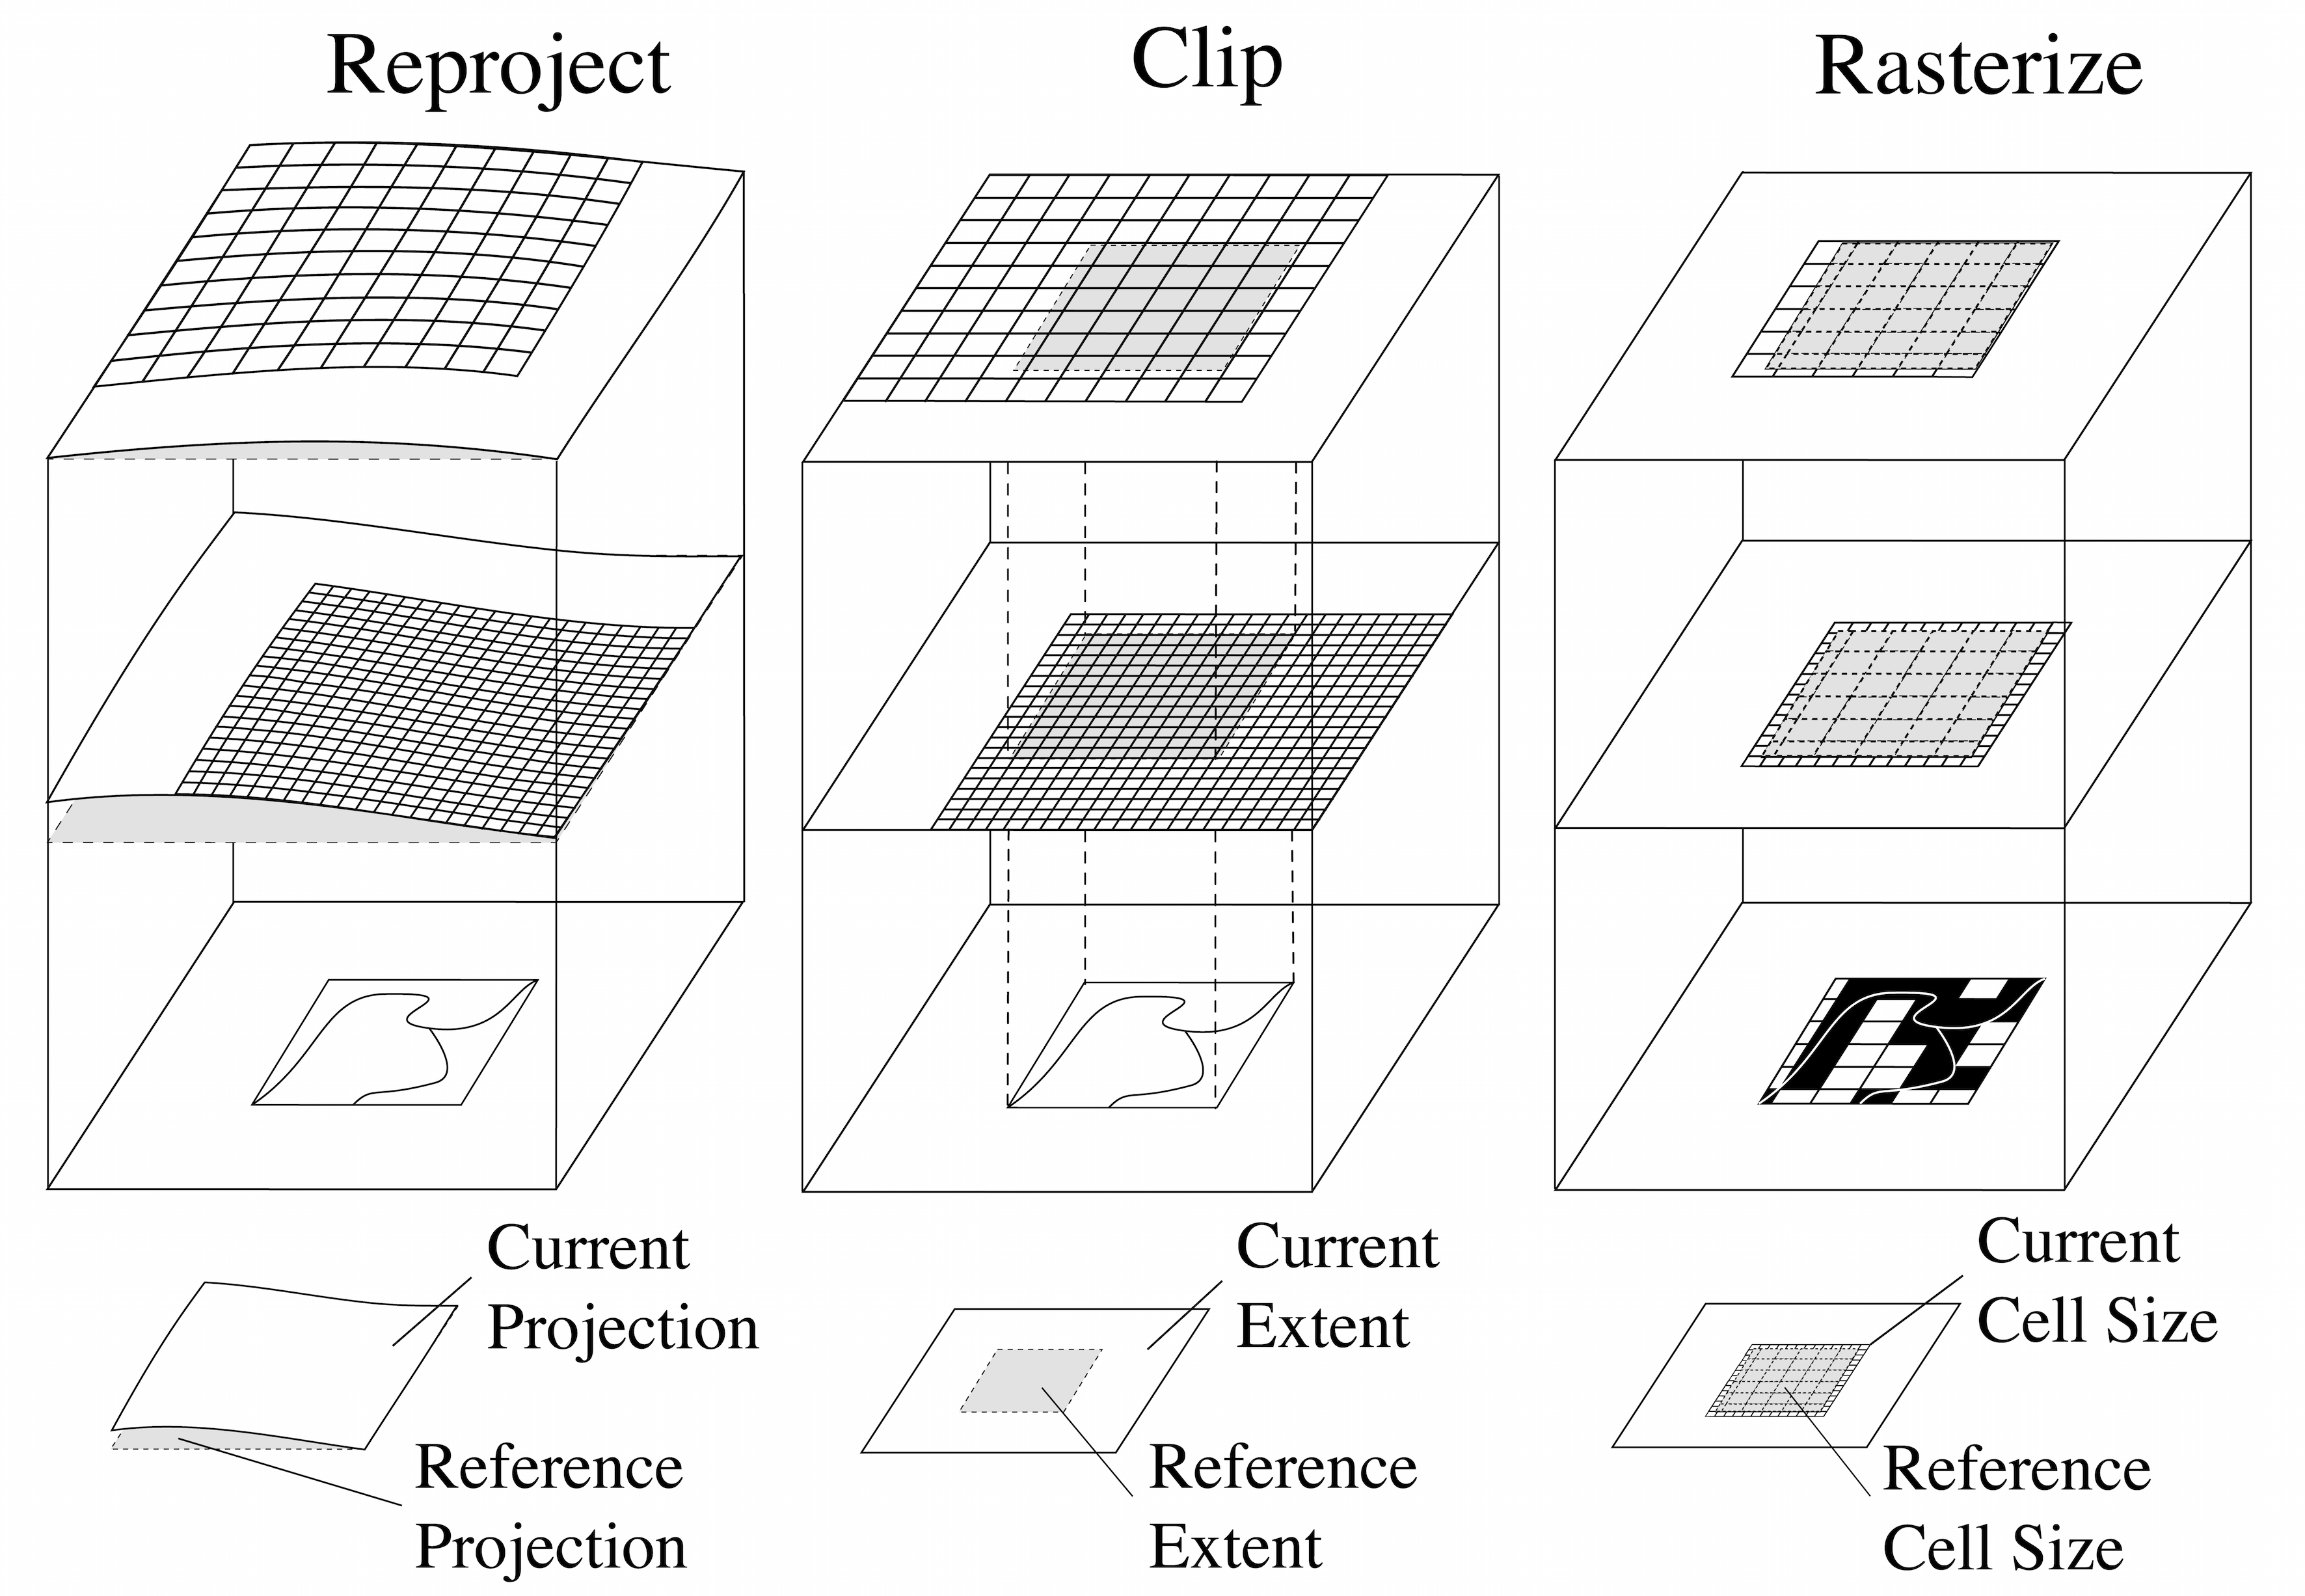
\includegraphics[width=5.5in]{figures/data-processing-workflow.png}
             \caption{Conceptual illustration of the input data preprocessing operations and workflow phases typical to most MCSS analyses}
              \label{fig:Preprocessing}
              \end{center}
        \end{figure} 
        
\section{Workflow Automation}
    
The overarching goal of the software development effort was to functionalize as many components of this generic data preprocessing workflow as possible within the MATLAB$^{\circledR}$ environment. In light of this objective, the control flow logic guiding the implementation of the toolset is described in the pseudocode contained within ~Figure \ref{fig:Pseudocode}. 

Prior to the initiation of this process the user must provide a set of raw spatial data input files and designate a set of spatial reference criteria. Once these requirements are met, all of the input spatial data files are then looped over and subjected to a sequence of conditional statements. Depending upon the result of these conditional statement evaluations various transformation functions are then sequentially applied to the input data files so as to produce a set of outputs whose projection, spatial extent, cell size, and cell alignment all match a set of designated spatial reference criteria.



                \begin{algorithm}
                \caption{}\label{euclid}
                \begin{algorithmic}[1]
                    \Procedure{Preprocess Input Data}{}
                        \ForAll{$input$}
                            \If{$input_{prj} \neq reference_{prj}$}
                                \State $input = Reproject(input)$
                            \ElsIf{$input_{ext} \neq reference_{ext}$}
                                \State $input = Clip(input)$
                            \ElsIf{$ isRaster(input_{type}) \neq True$}
                                \State $input = Rasterize(input)$
                            \ElsIf{$input_{cs} \neq reference_{cs}$}
                                \State $input = Resize(input)$
                            \EndIf
                            \State $output = input$
                        \EndFor
                        \State \textbf{return} $output$
                    \EndProcedure
                \end{algorithmic}
                \end{algorithm}
                
            \begin{figure}[WOGRSS Data Preprocessing Algorithm Pseudocode]
            \caption[WOGRSS Data Preprocessing Algorithm Pseudocode]{WOGRSS Data Preprocessing Algorithm Pseudocode}
            \label{fig:wogrss-pseudocode}
            \end{figure}

            
One feature of note is that the current iteration of the toolset only supports the reprojection of input spatial data layers that are represented using geographic coordinates -- i.e. data stored in latitude \& longitude coordinate space). This constraint not only limits the directionality of the reprojection operation but also greatly simplifies the code which is used to implement the spatial interpolation routines required for the rasterization process. The authors plan to lift this restriction in future iterations of the toolset as the MATLAB$^{\circledR}$ language's native support for forward map projection as well as the automated parsing of standard formatted spatial reference data strings improves over time.   
            
\section{MCSS Computation}
            
Following the preprocessing of the spatial data inputs, the next major phase of the MCSS modeling process is the user guided reclassification of the data values in each layer such that they are transformed into a quantitative measure of suitability for the land use application in question. A number of interactive routines are provided in the toolset to facilitate this process. Among these included an automated histogram equalization based reclassification procedure which assigns suitability values in such a way as to ensure an even distribution of all the values contained within some range across all of the areas within the spatial data layer. In addition to this, other more interactive tools are provided, which allow the user to manually specify the range of the bins used for the reclassification of raw input data values to site suitability rankings. 

\section{Software Toolset Repository Architecture}
    
The software tools which have been developed in conjunction with this research program are publicly available via the GitHub repository hosted at the following URL: \url{https://github.com/ericdfournier/WOGRSS}. The directory structure of this repository is illustrated in ~Figure \ref{fig:Directory}. Below the top level root directory are four standalone files: (1) a \textit{\textbf{LICENSE.md}} file, (2) a \textit{\textbf{README.md}} file, (3) a \textit{\textbf{MAIN.m}} file, and (4) a \\textit{textbf{GUI.app}} file. The first two files contain the software license and general repository usage guidance, respectively. The third, \textit{\textbf{MAIN.m}}, is a script which provides an example of how to chain the included functional routines in such a way so as to achieve the goals of the data preprocessing workflow previously described. The fourth, \textit{\textbf{GUI.app}}, is a compiled executable containing a standalone graphical user interface that visually guides a user through this same data preprocessing workflow.

        \begin{figure}[!h]
            \dirtree{%
             .1 $\dots$/.
             .2 LICENSE.md.
             .2 README.md.
             .2 MAIN.m.
             .2 GUI.app.
             .2 src/.
             .3 *.m (functions).
             .2 prm/.
             .3 *.m (scripts).
             .2 input/.
             .3 vector/.
             .4 *(filename)/.
             .5 *.shp, *.shx, *.dbf, *.prj.
             .3 raster/.
             .4 *(filename)/.
             .5 *.tif, *.tfw.
             .2 output/.
             .3 binary/.
             .4 *.mat.
             .3 raster/.
             .4 *.tif, *.tfw.
            }
            \caption{Directory tree structure for the toolset repository. Filetypes required for input data and automatically generated as output data are shown.}
              \label{fig:Directory}
        \end{figure}
        
Also below the top level root directory are the following four subdirectories: (1) \textit{\textbf{src/}}, (2) \textit{\textbf{prm/}}, (3) \textit{\textbf{input/}}, and (4) \textit{\textbf{output/}}. The \textit{\textbf{src/}} directory contains the MATLAB$^{\circledR}$ source code m-files comprising the toolset's various functions. The \textit{\textbf{prm/}} directory contains MATLAB$^{\circledR}$ .m-file scripts \& that can optionally be called to automate the execution of multiple data preprocessing workflows. The \textit{\textbf{input/}} directory contains two sub-directories: \textit{\textbf{vector/}} and \textit{\textbf{raster/}}. Each of these houses the corresponding sub-directories, one for each vector and raster based raw input spatial data files provided by the user. The tiles used for each of these \textit{\textbf{*(filename)}} sub-directories are the ones which shall be used for the outputs generated by the tool. The supported vector input filetype is the ESRI shapefile format. Alternatively, the supported raster input file type is the open source GeoTiff format. Finally, the \textit{\textbf{output/}} directory contains two sub-directories: \textit{\textbf{binary/}} and \textit{\textbf{raster/}}. These subdirectories comprise the default destination locations for all of the outputs generated by the toolset tools. Outputs can be produced in either the mat-file MATLAB$^{\circledR}$ ASCII-binary format or in the same GeoTiff format as the input raster data.

One feature of note with respect to the previously mentioned requirements regarding the format of the input data sources is that the toolset supports the use of composite raster data sets which are made up of multiple, possibly overlapping, individual raster data tiles. It does this by performing a bounding box intersection test for each input raster data tile with the reference spatial domain. For those tiles whose bounding boxes are found to intersect with that of the reference domain, values are iteratively compiled into a new composite mosaic data layer made up of, potentially several, individual tiles. This feature of the toolset makes it possible to use input raster data layers that are of arbitrarily high resolution covering large geographic domains.
    


    \section{Sample Input Data Sources}
    
The raw input datasets which were selected for the case study implementation were collected from a diverse array of publicly available sources. A brief topical description of each source as well as a link to the source web repository for each is referenced in the table contained in ~Figure \ref{fig:DataSources}. In addition to these raw input data sources, a number of derived data products are generated automatically from the digital elevation model (DEM) for use in this particular case study analysis. These derived products include: slope, aspect, and gradient (North \& South).

    \begin{figure}[!h]
        \begin{center}
            \begin{tabular*}{0.45\textwidth}{| l | l | l |}
                \textbf{Type} & \textbf{Category} & \textbf{Source} \\ \hline
                Vector & Resource Areas & \href{http://www.atlas.ca.gov/download.html}{Cal-Atlas} \\ \hline
                Vector & County Boundaries & \href{http://www.atlas.ca.gov/download.html}{Cal-Atlas} \\ \hline
                Vector & Surface Geology & \href{http://mrdata.usgs.gov/geology/state/state.php?state=CA}{USGS} \\ \hline
                Vector & Road Network & \href{http://www.atlas.ca.gov/download.html}{Cal-Atlas} \\ \hline
                Vector & STATSGO Soils & \href{http://water.usgs.gov/GIS/metadata/usgswrd/XML/ussoils.xml#stdorder}{USGS} \\ \hline
                Vector & State Park Boundaries & \href{http://www.atlas.ca.gov/download.html}{Cal-Atlas} \\ \hline
                Vector & Stream Reaches & \href{http://viewer.nationalmap.gov/viewer/}{National Map} \\ \hline
                Vector & Street Network & \href{http://www.atlas.ca.gov/download.html}{Cal-Atlas} \\ \hline
                Vector & Surface Water Storage & \href{http://www.atlas.ca.gov/download.html}{Cal-Atlas} \\ \hline
                Raster & Crop Data Layer & \href{http://www.nass.usda.gov/research/Cropland/SARS1a.htm}{USDA} \\ \hline
                Raster & Digital Elevation Model & \href{http://viewer.nationalmap.gov/viewer/}{National Map} \\ \hline
                Raster & NLCD Landcover & \href{http://viewer.nationalmap.gov/viewer/}{National Map} \\ 
           \end{tabular*}
    \end{center}
    \caption{Table of input data sources used in the case study MCSS model for artificial groundwater recharge applications.}
    \label{fig:DataSources}
    \end{figure}

\section{Geographic Unit of Analysis}
    
    The geographic unit of analysis selected for this case study implementation is the US Geologic Survey (USGS) Hydrologic Unit Code (HUC) level five watershed. Specifically, the level five watershed areas contained within the administrative boundaries of the state of California. According to the USGS: 
    \blockquote{\textit{The United States is divided and sub-divided into successively smaller hydrologic units which are classified into four levels: regions, sub-regions, accounting units, and cataloging units. The hydrologic units are arranged or nested within each other, from the largest geographic area (regions) to the smallest geographic area (cataloging units). Each hydrologic unit is identified by a unique HUC consisting of two to twelve digits based on the levels of classification in the hydrologic unit system. \cite{Seaber1987}}}
    The level five designation within this HUC framework is comprised of closed contiguous regions possessing an average area of $227$ square miles. These level five HUC designated areas are often referred to as HUC-10 watersheds because of their use of a ten digit unique numerical identification code. Within the state of California, there are 1,040 individual HUC-10 watersheds. These watersheds are non-overlapping and have been derived algorithmically from the national elevation dataset by USGS scientists according to the method described by \cite{Seaber1987}.
    
\section{WOGRSS Outputs}
    
    ~Figure \ref{fig:SampleOutput} illustrates a set of sample outputs that were generated by the data preprocessing components of the toolset for a single HUC-10 reference boundary selected, arbitrarily, for the purpose of illustration. The selection of this reference boundary can either be achieved manually, by calling a function which prompts the user to click on map with all of the HUC-10 boundaries drawn on it, or automatically, be specifying the 10-digit code corresponding to the desired HUC-10 watershed. Following the execution of these toolset processes an output layer stack is generated -- the individual component layers of which are illustrated in the colored inset map panels. Only layers for which there is at least one non-empty data value are included in the generated outputs. Thus, the number of components of this output may vary depending upon the coverage of the input data layers relative to the domain of the reference boundary. For vector data inputs, the values which are contained in the output are those corresponding to a single attribute field selected by the user. This field must be coded as a either a real or coded numeric data type as the raster data format does not support the native representation of categorical variables.
    
        \begin{figure}[!h]
            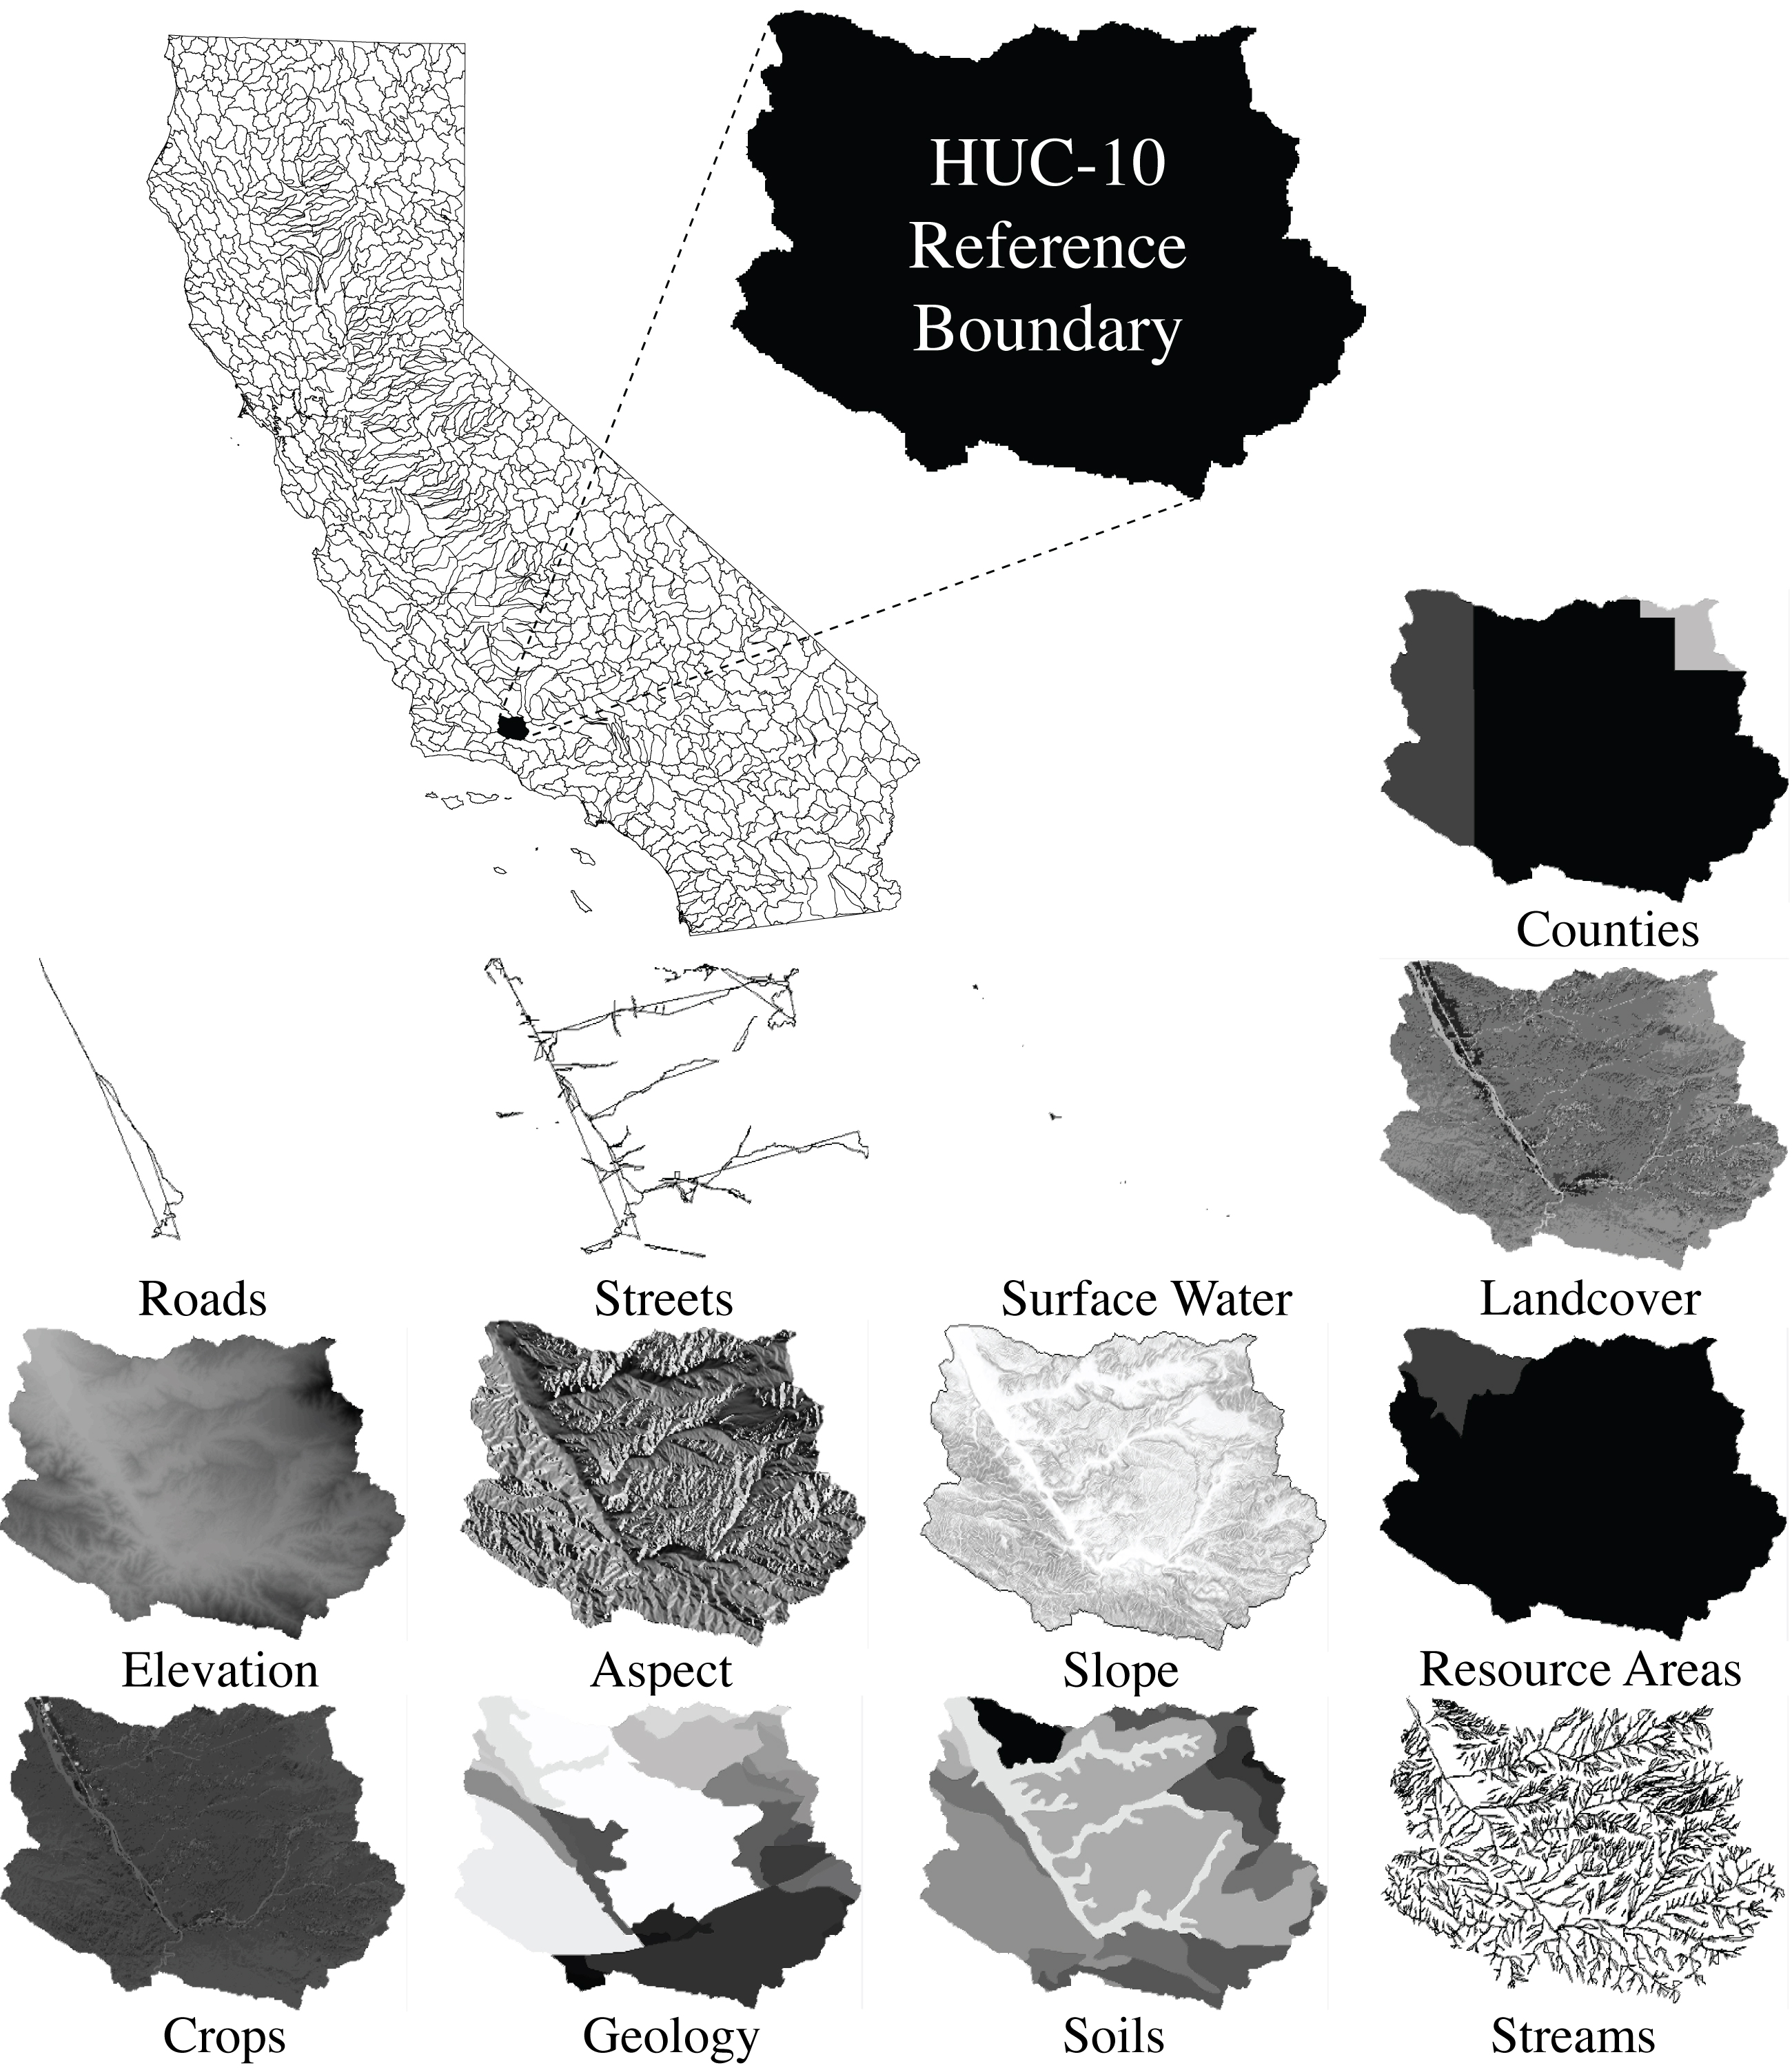
\includegraphics[width=5.5in]{figures/example_data_output.png}
            \caption{A graphical illustration of the sample outputs generated by the data preprocessing toolset for an arbitrarily selected HUC-10 watershed within the State of California. Shown in each of the colored panels are the individual layers contained in the output layer stack generated for selected HUC-10 reference boundary. These layers have been projected, clipped, and rasterized and ready for use in an MCSS analysis.}
            \label{fig:SampleOutput}
        \end{figure}

    An important feature of the way in which this toolset has been structured is that it allows for the automated repetition of this data preprocessing workflow for a large number of reference boundaries. In this case study implementation, for example, the tool was used to prepare a single such output layers stack for each of the 1,040 individual HUC-10 reference boundaries contained within the state of California. With these outputs, a corresponding the MCSS analysis could then be easily conducted for any or every such HUC-10 watershed in the State. 
   
\section{Conclusions}

    This note introduces a set of software tools written in the MATLAB$^{\circledR}$ programming language which enable the automated preprocessing of large and heterogeneous input spatial data sources for use in MCSS analyses. The availability of this toolset provides the opportunity for researchers to more tightly couple GIS type spatial data manipulation operations with dedicated numerical modeling routines. While, the case study implementation detailed in the paper focuses on the preprocessing of heterogeneous spatial data layers for use in MCSS type analyses, it is quite possible that the provided functions could be adapted to facilitate any numerical modeling procedure involving the use of structure raster data layers.
    